\documentclass{article}

\usepackage{amsmath,amsfonts,latexsym,graphicx}
\usepackage{fullpage,color}
\usepackage{setspace}
\usepackage{float}

\usepackage{tocloft}
\setlength{\cftbeforesecskip}{10pt}
\renewcommand{\cftbeforesubsecskip}{4pt}
\renewcommand{\cftbeforesubsubsecskip}{4pt}
\renewcommand\cftdotsep{2}
\setcounter{secnumdepth}{4}
\setcounter{tocdepth}{4}

\usepackage{fancyhdr}
\usepackage{hyperref}

\usepackage{xeCJK}

\usepackage{indentfirst}
\setlength{\parindent}{2em}

\usepackage[linesnumbered,boxed,ruled,vlined]{algorithm2e}

\usepackage{textgreek}

\begin{document}
\begin{titlepage}
\fancyhead[CH]{}

\hspace{3.0cm}
\begin{center}
\vfill
% Upper part of the page

\textsc{\LARGE Tsinghua University}\\[1.5cm]

\textsc{\Large Computer Organization Experimentation}\\[0.5cm]


% Title
\rule[0.75\baselineskip]{0.75\textwidth}{1pt}

{ \huge \bfseries Design Description}\\[0.4cm]

\rule[20\baselineskip]{0.75\textwidth}{1pt}

% Author and supervisor
\begin{minipage}{0.4\textwidth}
\begin{flushleft} \large
\emph{Author:}\\
Shizhi \textsc{Tang}

Xihang \textsc{Liu}

Zixi \textsc{Cai}
\end{flushleft}
\end{minipage}
\begin{minipage}{0.4\textwidth}
\begin{flushright} \large
\emph{Supervisor:} \\
Yuxiang \textsc{Zhang}

Prof.~Weidong \textsc{Liu}
\end{flushright}
\end{minipage}

\vfill
\vspace{3.0cm}
% Bottom of the page
{\large \today}

\end{center}

\end{titlepage}
\setcounter{page}{2}
\tableofcontents
\newpage
\begin{spacing}{1.4}

%%%%%%%%%%%%%%%%%%%%%%
%     BODY BEGIN     %
%%%%%%%%%%%%%%%%%%%%%%

\section{概述}

本文是MIPS32 CPU设计nCore的设计文档。

\subsection{常量}

本文中所使用的常量定义如Table~\ref{tb:constants}。
\begin{table}[!htb]
\begin{center}
\begin{tabular*}{15cm}{l|l|p{10cm}}  
\hline  
\textbf{常量}&\textbf{值}&\textbf{功能} \\
\hline InstWidth            & 31..0    & 指令宽度 \\
\hline DataWidth            & 31..0    & 数据宽度 \\
\hline AddrWidth            & 31..0    & 地址宽度 \\
\hline StallWidth           & 5..0     & 暂停信号宽度,每个分量对应一个需要被暂停的客体 \\
\hline ExceptionCauseWidth  & 4..0     & 异常编号的宽度 \\
\hline 
\end{tabular*}  
\caption{常量}
\label{tb:constants}
\end{center}
\end{table}

\subsection{文档结构}

本文按以下结构组织:首先介绍整体的层次划分。对于每一层次,介绍其实体\footnote{实体即VHDL中的entity或Verilog中的module}划分,然后依次介绍各实体。对于每个实体,分别介绍其功能、参数\footnote{参数即VHDL中的generic或Verilog中的parameter,是编译期确定的,用于方便地生成用于不同环境,例如功能测例、\textmu Core和u-boot,的目标逻辑}(如有)、接口和具体设计。

\section{层次划分}

nCore自底向上分为三个层次:数据通路、访存控制和I/O。数据通路层是nCore的核心,此层实现了标准的MIPS五级流水线和CP0协处理器,及其所需的数据旁路、暂停、异常等机制的控制逻辑。访存控制层解决了指令访存和数据访存的结构冲突,将其封装为统一的访存逻辑。I/O层则将统一的访存按不同外设的性质特化。这三层间的数据流关系见Figure~\ref{fig:layer-data-flow}。

\begin{figure}[!htb]
	\centering
	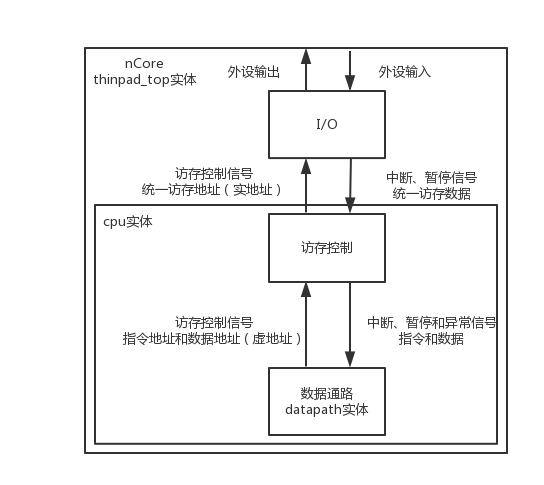
\includegraphics[width=.7\textwidth]{layer-data-flow.png}
	\caption{各层次间的数据流}
    \label{fig:layer-data-flow}
\end{figure}

各层次用组合(Composition)的方式例化,下层实体例化与上层实体中。具体地,数据通路层实现于datapath实体中;访存控制实现于cpu实体中,但cpu实体中也例化了datapath实体;I/O实现于thinpad\_top实体中,但thinpad\_top实体中也例化了cpu实体。像这样将下层实体直接例化在上层实体中,而不是在顶层实体中连接所有层,减少了层间的冗余连接,也对下层实体进行了很好的封装。

下文将依次介绍各个层次。此外,少数实体在逻辑上不属于这三层中的任意一层,例如时钟驱动器,但在实现中例化于某一层的顶层实体中,也将于该层一并介绍。

\section{数据通路层}

\subsection{概述}

数据通路层以MIPS五级流水线为核心。实体id、ex、mem分别实现了译码、执行、访存阶段,实体if\_id、id\_ex、ex\_mem、mem\_wb分别实现了取指/译码、译码/执行、执行/访存、访存/写回间的阶段寄存器。取指和写回阶段不实现于单独的实体:取指逻辑主要实现于程序计数器(PC)实体;写回逻辑由被写入的目标处理,这些目标包括寄存器堆、CP0协处理器、乘除法HI/LO寄存器。实体ctrl通过控制各阶段寄存器实现流水线的暂停和清空(处理异常时)。此外,除法逻辑实现于单独的实体。

本层包含的所有实体见Table~\ref{tb:datapath-entities}:

\begin{table}[!htb]
\begin{center}
\begin{tabular}{p{7.5cm}|p{7.5cm}}  
\hline  
\textbf{实体}&\textbf{功能} \\
\hline datapath & 顶层实体 \\
\hline pc\_reg & 程序计数器(PC) \\
\hline if\_id & 取指/译码阶段寄存器 \\
\hline regfile & 通用寄存器堆 \\
\hline id & 译码阶段 \\
\hline id\_ex & 译码/执行阶段寄存器 \\
\hline ex & 执行阶段 \\
\hline div & 除法器 \\
\hline ex\_mem & 执行/访存阶段寄存器 \\
\hline mem & 访存阶段 \\
\hline mem\_wb & 访存/写回阶段寄存器 \\
\hline hi\_lo & 乘除法HI/LO寄存器 \\
\hline ctrl & 流水线控制器 \\
\hline cp0\_reg & CP0协处理器 \\
\hline 
\end{tabular}  
\caption{数据通路层的实体}
\label{tb:datapath-entities}
\end{center}
\end{table}

\subsection{整体设计}

正常情况下,数据沿流水线逐级传递并加工。数据通路层各实体间的主要数据流见Figure~\ref{fig:datapath-data-flow},其中实线表示正常数据流,虚线表示旁路数据流。

\begin{figure}[!htb]
	\centering
	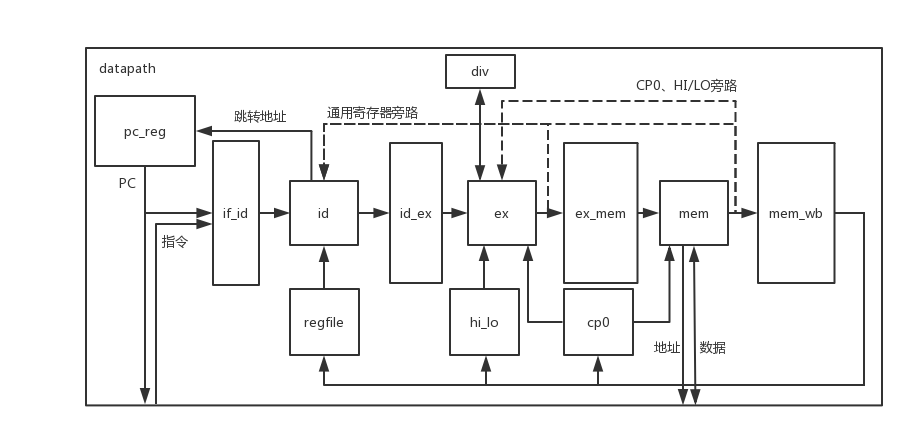
\includegraphics[width=\textwidth]{datapath-data-flow.png}
	\caption{数据通路层数据流}
    \label{fig:datapath-data-flow}
\end{figure}

当有异常发生时,每个阶段将该阶段发生的异常逐级传递至访存阶段。访存阶段根据CP0控制信息向ctrl实体发出异常请求,ctrl实体命令各阶段寄存器进行清空,并修改PC以跳转至异常处理向量。异常处理的控制流见Figure~\ref{fig:datapath-exception-flow}。

\begin{figure}[!htb]
	\centering
	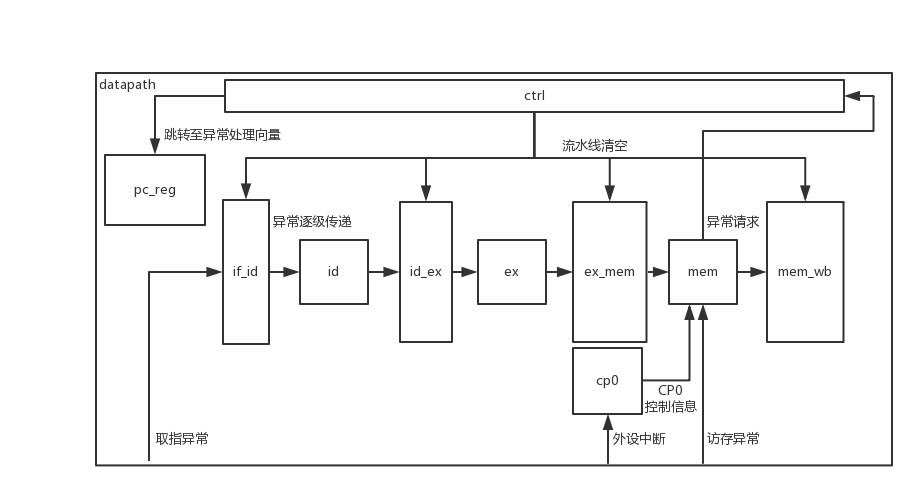
\includegraphics[width=\textwidth]{datapath-exception-flow.png}
	\caption{异常控制流}
    \label{fig:datapath-exception-flow}
\end{figure}

当需要流水线暂停(插入空泡)时,需要暂停的主体向ctrl实体发出暂停请求,ctrl实体命令各阶段寄存器进行暂停。暂停控制流见Figure~\ref{fig:datapath-stall-flow}。

\begin{figure}[!htb]
	\centering
	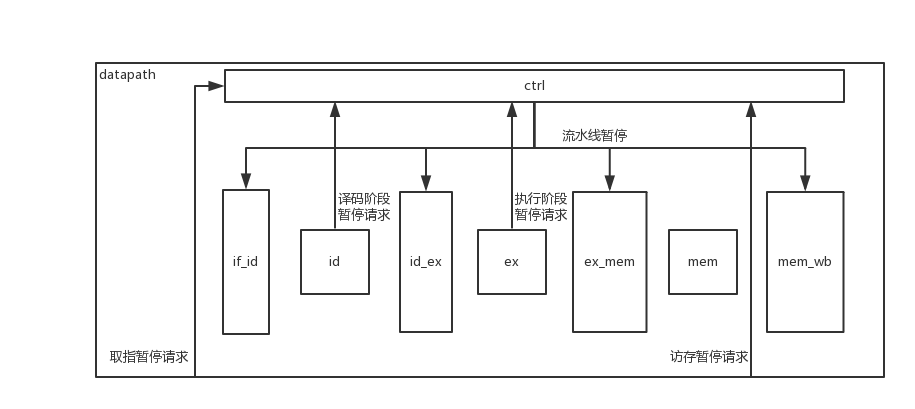
\includegraphics[width=\textwidth]{datapath-stall-flow.png}
	\caption{暂停控制流}
    \label{fig:datapath-stall-flow}
\end{figure}

\subsection{各实体说明}

以下介绍除数据通路层除顶层实体外的各实体。顶层实体datapath的说明见上层(访存控制层)。

\subsubsection{pc\_reg}

\paragraph{功能}\mbox{}

pc\_reg实现了程序计数器(PC)的寄存器。PC中储存了当前处于取指阶段指令的地址。每个周期PC会发生改变,根据pc\_reg的输入,改变分为顺序执行、分支/跳转、异常跳转三种情况。

\paragraph{参数}\mbox{}

pc\_reg实体的参数定义见Table~\ref{tb:pcreg-parameter}。
\begin{table}[!htb]
\begin{center}
\begin{tabular*}{15cm}{l|l|l}  
\hline  
\textbf{参数}&\textbf{类型}&\textbf{功能} \\
\hline instEntranceAddr        & std\_logic\_vector(AddrWidth)    & 重置后PC的值 \\
\hline 
\end{tabular*}  
\caption{pc\_reg实体的参数}
\label{tb:pcreg-parameter}
\end{center}
\end{table}

\paragraph{接口}\mbox{}

pc\_reg实体的接口定义见Table~\ref{tb:pcreg-interface}。
\begin{table}[!htb]
\begin{center}
\begin{tabular*}{15cm}{l|l|l|l|p{5cm}}  
\hline  
\textbf{信号}&\textbf{宽度}&\textbf{I/O}&\textbf{来源/去向}&\textbf{功能} \\
\hline rst                     & 1             & I     & 上层          & 同步重置 \\
\hline clk                     & 1             & I     & 上层          & 时钟 \\
\hline stall\_i                & StallWidth    & I     & ctrl          & 对应pc\_reg的分量为高电平表示需要暂停 \\
\hline branchTargetAddress\_i  & AddrWidth     & I     & id            & 跳转目标 \\
\hline branchFlag\_i           & 1             & I     & id            & 高电平表示需要跳转 \\
\hline flush\_i                & 1             & I     & ctrl          & 高电平表示发生了异常 \\
\hline newPc\_i                & AddrWidth     & I     & ctrl          & 异常处理向量 \\
\hline pc\_o                   & AddrWidth     & O     & if\_id, 上层  & PC \\
\hline pcEnable\_o             & 1             & O     & if\_id        & 高电平表示此指令不是空泡 \\
\hline 
\end{tabular*}  
\caption{pc\_reg实体的接口}
\label{tb:pcreg-interface}
\end{center}
\end{table}

\paragraph{设计}\mbox{}

每个时钟上升沿,若发生了异常,则置PC为异常处理向量,否则判断取指阶段是否被暂停。若被暂停,则PC不变;若未被暂停,则判断是否发生了分支/跳转。若是,则置PC为分支/跳转目标,否则置PC为下一条指令地址(PC+4)。

其中,在判断分支/跳转时,正常情况下,表示是否跳转以及跳转目标的信号来自译码阶段。但是若上一个周期取指阶段被暂停了,此周期译码阶段会是空泡,导致接收不到上述信号。故pc\_reg会在取指暂停时依旧接收跳转相关信号并保存之,待恢复执行后使用。

\subsubsection{if\_id}

\paragraph{功能}\mbox{}

if\_id是取指阶段与译码阶段间的阶段寄存器,用于保存某个周期取指的结果,在下一个周期交予译码阶段。作为阶段寄存器,if\_id会接受ctrl实体的控制。

\paragraph{接口}\mbox{}

if\_id实体的接口定义见Table~\ref{tb:ifid-interface}。
\begin{table}[!htb]
\begin{center}
\begin{tabular*}{15cm}{l|l|l|l|p{5cm}}
\hline
\textbf{信号}&\textbf{宽度}&\textbf{I/O}&\textbf{来源/去向}&\textbf{功能} \\
\hline rst                     & 1                      & I     & 上层          & 同步重置 \\
\hline clk                     & 1                      & I     & 上层          & 时钟 \\
\hline pc\_i                   & AddrWidth              & I     & pc\_reg       & PC \\
\hline instEnable\_i           & 1                      & I     & pc\_reg       & 高电平表示此指令不是空泡 \\
\hline inst\_i                 & InstWidth              & I     & 上层          & 指令 \\
\hline exceptCause\_i          & ExceptionCauseWidth    & I     & 上层          & 取指异常类型或无异常 \\
\hline pc\_o                   & AddrWidth              & O     & id            & PC \\
\hline valid\_o                & 1                      & O     & id            & 高电平表示此指令不是空泡 \\
\hline inst\_o                 & InstWidth              & O     & id            & 指令 \\
\hline exceptCause\_o          & ExceptionCauseWidth    & O     & id            & 取指异常类型或无异常 \\
\hline stall\_i                & StallWidth             & I     & ctrl          & 对应if\_id的分量为高电平表示需要暂停 \\
\hline flush\_i                & 1                      & I     & ctrl          & 高电平表示流水线需要清空 \\
\hline
\end{tabular*}
\caption{if\_id实体的接口}
\label{tb:ifid-interface}
\end{center}
\end{table}

\paragraph{设计}\mbox{}

若流水线需要清空,则输出零/无效信号;否则,若流水线暂停,则保持上一个周期的值;否则,将阶段寄存器的值置为来自取指阶段的值。

\subsubsection{regfile}
\subsubsection{id}
\subsubsection{id\_ex}
\subsubsection{ex}
\subsubsection{div}
\subsubsection{ex\_mem}
\subsubsection{mem}
\subsubsection{mem\_wb}
\subsubsection{hi\_lo}
\subsubsection{ctrl}
\subsubsection{cp0\_reg}

%%%%%%%%%%%%%%%%%%%%%%
%     BODY END       %
%%%%%%%%%%%%%%%%%%%%%%

\end{spacing}
\end{document}